\documentclass[12pt,a4paper]{article}

\usepackage[utf8]{inputenc}
\usepackage[T1]{fontenc}
\usepackage[french]{babel}
\usepackage{geometry}
\usepackage{graphicx}
\usepackage{float}
\usepackage{subcaption}
\usepackage{booktabs}
\usepackage{amsmath}
\usepackage{amssymb}
\usepackage{hyperref}
\usepackage{xcolor}
\usepackage{listings}
\usepackage{enumitem}

\geometry{margin=1.6cm}

\hypersetup{
    colorlinks=true,
    linkcolor=blue!60!black,
    urlcolor=blue!60!black,
    citecolor=blue!60!black
}

\lstset{
    basicstyle=\ttfamily\small,
    keywordstyle=\color{blue!70!black},
    commentstyle=\color{green!40!black},
    stringstyle=\color{red!60!black},
    frame=single,
    breaklines=true,
    columns=fullflexible,
    tabsize=4,
    language=C++
}

\title{\textbf{\Huge Projet Blob War}}

\author{Mohammed Akram Lrhorfi : équipe 17 : Dogue Dieyeneba}
\date{Mai 2026}

\begin{document}

\maketitle


\begin{figure}[h]
    \centering
    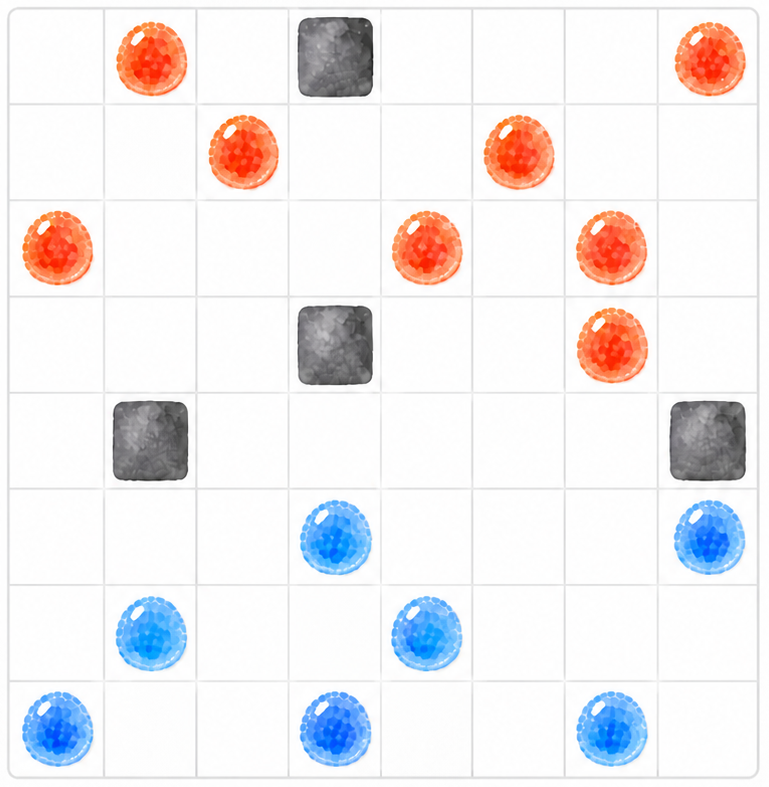
\includegraphics[width=0.7\textwidth]{image_blob_art}
\end{figure}

\begin{abstract}
Blob War est un jeu combinatoire a information parfaite sur un plateau $8 \times 8$. A chaque tour,
un joueur duplique ou deplace un pion, puis convertit les voisins adverses. Comme l'arbre de jeu croit
rapidement, une recherche exhaustive est impossible dans le temps du tournoi. Nous comparons donc une
strategie gloutonne, un Minimax a profondeur fixe, une version Alpha-Beta parallele intermediaire et
une version Alpha-Beta optimisee, en mesurant le temps par coup, la profondeur atteinte, les noeuds
explores, les coupures Alpha-Beta et le taux de victoire.
\end{abstract}

\newpage

\section{Modelisation du jeu}

\subsection{Etat du plateau}

Dans le code fourni, le plateau est represente par deux tableaux bidimensionnels :

\begin{itemize}[nosep]
    \item \texttt{bidiarray<Sint16> \_blobs} indique l'occupant de chaque case : $-1$ pour une case vide,
    sinon l'identifiant du joueur ;
    \item \texttt{bidiarray<bool> \_holes} indique les cases interdites ;
    \item \texttt{\_current\_player} stocke le joueur qui doit jouer.
\end{itemize}

Un coup est represente par la structure \texttt{movement}, qui contient les coordonnees d'origine
et de destination .

\subsection{Application d'un coup}

La fonction \texttt{applyMove()} simule les regles de Blob War. Elle distingue les deux types de
deplacements par la distance de Chebyshev :

\begin{itemize}[nosep]
    \item si la distance vaut $1$, le pion est duplique ;
    \item si la distance vaut $2$, la case source est videe ;
    \item la destination devient la propriete du joueur courant ;
    \item les voisins adverses de la destination sont convertis.
\end{itemize}

Dans les strategies, nous supposons que les coups donnes a \texttt{applyMove()} sont deja valides,
car ils proviennent de \texttt{computeValidMoves()}.

\subsection{Generation des coups}

La fonction \texttt{computeValidMoves()} parcourt tous les pions du joueur courant. Pour chaque pion,
elle examine les cases dans un carre de rayon $2$. Une case destination est acceptee si elle est dans
le plateau, non trouee, vide, et differente de la case source.

Si $b$ designe le nombre moyen de coups legaux, alors les algorithmes de recherche parcourent un arbre
de facteur de branchement approximatif $b$. A profondeur $d$, une recherche Minimax brute demande
donc de l'ordre de $O(b^d)$ noeuds.

\section{Strategies de recherche}

\subsection{Strategie gloutonne}

La strategie gloutonne est implementee dans \texttt{strategy\_glouton.cc}. Elle constitue notre
baseline. Pour chaque coup legal, elle simule le coup, evalue le plateau obtenu, puis conserve le
coup qui maximise le score.

\begin{lstlisting}
best_score = -INF
for mv in valid_moves:
    state = current_state
    state.applyMove(mv)
    score = state.estimateCurrentScore()
    if score > best_score:
        best_score = score
        best_move = mv
\end{lstlisting}


Cette strategie est tres rapide, car elle ne regarde qu'un coup en avant. Sa limite est qu'elle ne
tient pas compte des reponses adverses. Elle peut donc choisir un coup localement bon mais dangereux
au tour suivant.

\subsection{Minimax sequentiel}

Le Minimax est implemente dans \texttt{strategy\_minimax.cc}. Il explore l'arbre de jeu jusqu'a une
profondeur fixe, actuellement $d = 3$. Les noeuds du joueur courant maximisent le score, tandis que
les noeuds adverses le minimisent.

\begin{lstlisting}
minimax(state, depth, maximizing):
    if depth == 0:
        return evaluate(state)

    moves = validMoves(state)
    if moves.empty():
        return minimax(passTurn(state), depth - 1, !maximizing)

    if maximizing:
        return max(minimax(apply(mv), depth - 1, false))
    else:
        return min(minimax(apply(mv), depth - 1, true))
\end{lstlisting}

Le cas ou un joueur ne peut pas jouer est traite explicitement : on passe au joueur suivant. Si aucun
des deux joueurs ne peut jouer, l'etat est evalue directement.

La complexite theorique est :

\[
W_{minimax}(d) = O(b^d).
\]

Cette strategie anticipe mieux que le glouton, mais elle explore beaucoup de noeuds inutiles. Elle
sert donc de reference pour mesurer l'apport de l'elagage Alpha-Beta.

\subsection{Alpha-Beta parallele intermediaire}

La version intermediaire est implementee dans \texttt{strategy\_alphabeta0.cc}. Elle ajoute deux idees
importantes par rapport au Minimax :

\begin{itemize}[nosep]
    \item l'elagage Alpha-Beta ;
    \item la parallelisation des coups racine avec OpenMP.
\end{itemize}

L'algorithme Alpha-Beta conserve deux bornes :

\begin{itemize}[nosep]
    \item $\alpha$ : meilleure valeur garantie pour le joueur maximisant ;
    \item $\beta$ : meilleure valeur garantie pour le joueur minimisant.
\end{itemize}

Des qu'on obtient $\alpha \geq \beta$, le sous-arbre courant ne peut plus influencer la decision finale
et peut etre coupe.

\begin{lstlisting}
if alpha >= beta:
    return alpha   // coupure beta
\end{lstlisting}

Au niveau racine, les coups sont independants. Nous utilisons donc OpenMP :

\begin{lstlisting}
#pragma omp parallel for schedule(dynamic)
for (int i = 0; i < moveCount; i++) {
    Strategy child(*this);
    child.applyMove(moves[i]);
    score = child.alphaBeta(...);
}
\end{lstlisting}

Le choix \texttt{schedule(dynamic)} est important : deux sous-arbres de meme profondeur peuvent avoir
des couts tres differents selon les coupures Alpha-Beta. Une distribution dynamique par vol de travail equilibre donc mieux
le travail entre threads qu'une repartition statique.

\subsection{Alpha-Beta parallele optimise}

La strategie finale est implementee dans \texttt{strategy.cc}. Elle reprend Alpha-Beta et ajoute
plusieurs optimisations :

\begin{itemize}[nosep]
    \item tri des coups ;
    \item approfondissement iteratif ;
    \item sauvegarde immediate d'un coup valide ;
    \item sauvegarde apres chaque profondeur terminee ;
    \item partage d'une borne $\alpha$ atomique entre threads ;
    \item exploration sequentielle d'un prefixe de coups avant parallelisation du reste.
\end{itemize}

L'approfondissement iteratif permet de respecter la contrainte de temps du tournoi. Le processus de
recherche peut etre tue par le moteur apres le timeout ; il est donc essentiel d'avoir deja sauvegarde
un coup valide.

\begin{lstlisting}
bestMove = moves[0]
saveBestMove(bestMove)

for depth = INITIAL_SEARCH_DEPTH; ; depth++:
    depthBestMove = alphaBetaRoot(depth)
    bestMove = depthBestMove
    saveBestMove(bestMove)
\end{lstlisting}


\section{Heuristique d'evaluation}

\subsection{Heuristique materielle simple}

Les premieres strategies utilisent une evaluation simple :

\[
Material = pions_{moi} - pions_{adversaire}.
\]

Elle est pertinente en fin de partie, car le gagnant est determine par le nombre de pions. En revanche,
elle est pauvre en debut et milieu de partie : elle ne mesure ni la mobilite, ni la qualite positionnelle,
ni le risque de conversion au prochain tour.

\subsection{Heuristique multi-criteres}

Les versions Alpha-Beta utilisent une heuristique plus riche :

\[
Eval(s) =
w_m \cdot Material
+ w_{mob} \cdot Mobility
+ w_p \cdot Position.
\]

Le terme de mobilite est :

\[
Mobility = legalMoves(moi) - legalMoves(adversaire).
\]

Le terme positionnel repose sur une table de poids fixe. Les cases centrales ont un poids plus eleve, surtout sur la map \texttt{standard}. Pour le tournoi,
nous avons aussi ajoute une table adaptee a la map \texttt{x}, afin de favoriser les positions autour du trou central,
car elles offrent davantage de possibilites de deplacement et de conversion.

\begin{lstlisting}
static const int WEIGHT[8][8] = {
    {2, 3, 4, 4, 4, 4, 3, 2},
    {3, 4, 5, 6, 6, 5, 4, 3},
    {4, 5, 7, 8, 8, 7, 5, 4},
    {4, 6, 8, 10, 10, 8, 6, 4},
    {4, 6, 8, 10, 10, 8, 6, 4},
    {4, 5, 7, 8, 8, 7, 5, 4},
    {3, 4, 5, 6, 6, 5, 4, 3},
    {2, 3, 4, 4, 4, 4, 3, 2}
};
\end{lstlisting}

\subsection{Ponderation selon la phase de jeu}

L'heuristique s'adapte selon le nombre de cases vides :

\begin{lstlisting}
if (empty * 5 < playable) {
    return 220 * material + mobility;
}

if (empty * 2 > playable) {
    return 115 * material + 3 * mobility + 4 * positionBalance;
}

return 145 * material + 2 * mobility + 3 * positionBalance;
\end{lstlisting}

En debut de partie, la mobilite et la position sont importantes. En fin de partie, le materiel devient
dominant, car le score final depend directement du nombre de pions.

\subsection{Tri des coups}

Le tri des coups est une optimisation centrale pour Alpha-Beta. En effet, Alpha-Beta ne change pas le
resultat du Minimax, mais son efficacite depend fortement de l'ordre d'exploration. Avec un mauvais
ordre, le cout reste proche de :

\[
O(b^d).
\]

Avec un ordre presque optimal, Alpha-Beta peut approcher :

\[
O(b^{d/2}).
\]

Dans notre code, \texttt{moveOrderingScore()} favorise :

\begin{itemize}[nosep]
    \item les duplications ;
    \item les coups qui convertissent beaucoup de pions adverses ;
    \item les destinations ayant un bon poids positionnel.
\end{itemize}

\section{Parallelisation }

\subsection{Travail et profondeur}

Dans les algorithmes de recherche, on distingue deux mesures de complexite :
\begin{itemize}[nosep]
    \item le travail $W$, c'est-a-dire le cout total sur un processeur ;
    \item la profondeur $D$, c'est-a-dire la longueur du chemin critique.
\end{itemize}

Sur $p$ processeurs, la loi de Brent donne l'intuition suivante :

\[
T_p \approx \frac{W}{p} + D.
\]

Dans Blob War, le Minimax pur a un travail tres eleve, de l'ordre de $O(b^d)$. Le but d'Alpha-Beta
est de diminuer le travail effectif $W$ en coupant des sous-arbres. Le but de la parallelisation est
ensuite de repartir le travail restant entre plusieurs coeurs.

\subsection{Pourquoi Alpha-Beta est difficile a paralleliser}

Alpha-Beta contient une dependance sequentielle : les bornes $\alpha$ et $\beta$ sont mises a jour
apres chaque coup explore. Une boucle parallele naive peut donc explorer trop de sous-arbres avant
d'avoir une bonne borne.

\begin{lstlisting}
for mv in moves:
    score = search(mv, alpha, beta)
    alpha = max(alpha, score)
    if alpha >= beta:
        break
\end{lstlisting}

Le \texttt{break} montre que l'algorithme n'est pas naturellement un \texttt{for//} parfait. Il faut
paralleliser de facon speculative mais controlee.

\subsection{Strategie cascade }

Dans la strategie finale, nous explorons d'abord un prefixe des meilleurs coups sequentiellement.
La taille de ce prefixe est :

\[
k = \max(1, \lfloor \sqrt{b} \rfloor).
\]

Cette premiere phase donne une meilleure valeur de $\alpha$. Ensuite, les autres coups sont explores
en parallele avec une borne initiale plus forte.

\begin{lstlisting}
sequentialCount = sqrt(moveCount)

for i in 0..sequentialCount-1:
    search moves[i] sequentially
    update alpha

#pragma omp parallel for schedule(dynamic)
for i in sequentialCount..moveCount-1:
    search moves[i] in parallel
\end{lstlisting}

Cette idee est proche des algorithmes en cascade : on traite une petite partie du probleme
avec une methode plus sequentielle pour reduire le travail inutile, puis on exploite le parallelisme
sur le reste.

L'objectif de ce prefixe sequentiel est proche d'un \emph{killer move} : obtenir rapidement une bonne borne pour provoquer plus de coupures et reduire le travail des autres threads.

\section{Instrumentation et protocole experimental}

\subsection{Traces d'execution}

Chaque strategie affiche une ligne de trace au format suivant :

\begin{lstlisting}
BW_TRACE algo=alphabeta_final depth=5 nodes=123456 cutoffs=7890
\end{lstlisting}

Ces traces permettent de mesurer :

\begin{itemize}[nosep]
    \item la profondeur atteinte ;
    \item le nombre de noeuds explores ;
    \item le nombre de coupures Alpha-Beta ;
    \item le temps moyen par coup ;
\end{itemize}

Les experiences sont effectuees sur la carte \texttt{standard}, avec un timeout de $2$ secondes par
coup. Chaque algorithme joue contre chaque autre, dans les deux ordres : une partie ou le premier
algorithme commence, puis une partie ou le second commence.

\begin{lstlisting}[language=bash]
python3 benchmark_blobwar.py --timeout 2 --games-per-pair 1
\end{lstlisting}


\section{Resultats experimentaux}


\subsection{Temps moyen par coup}

\begin{figure}[H]
    \centering
    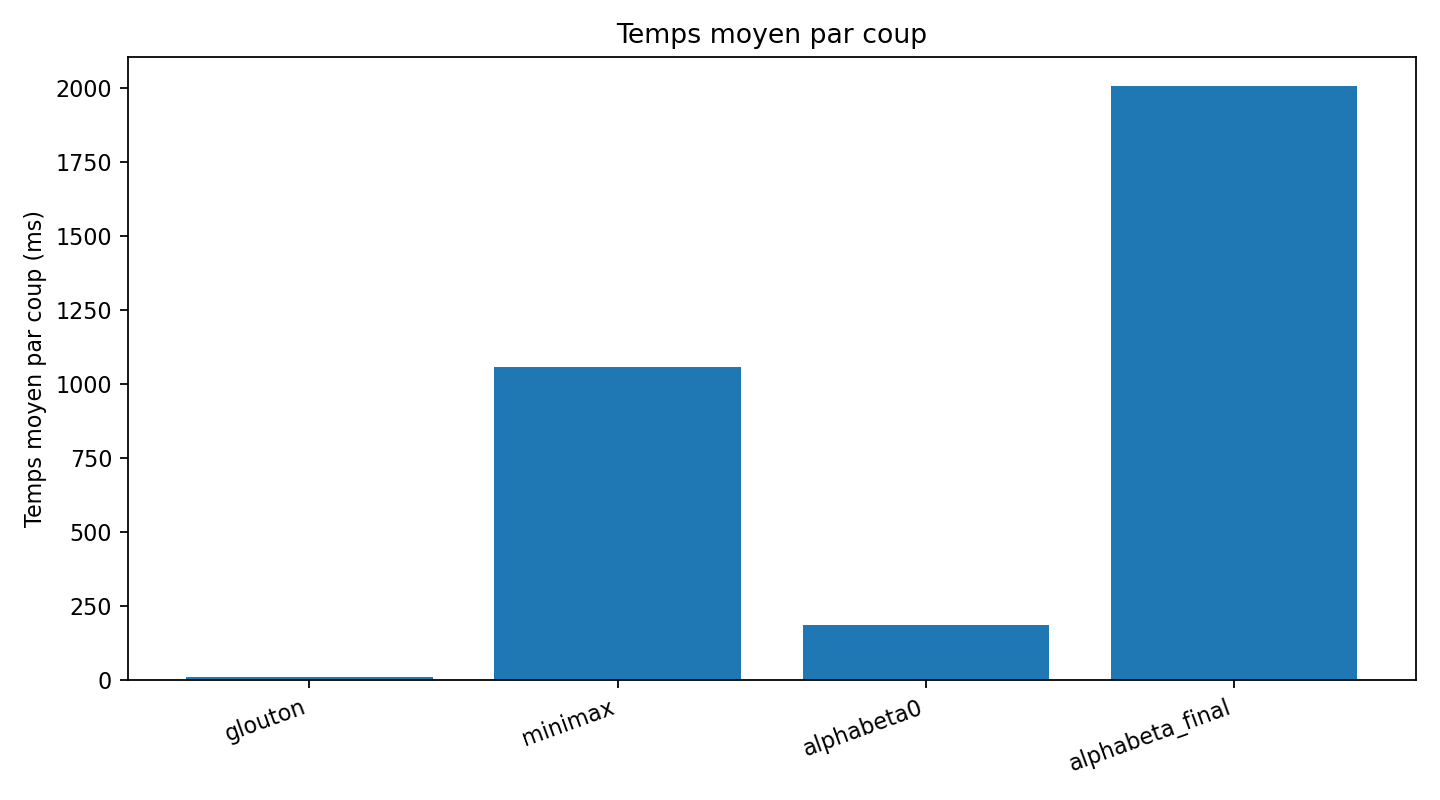
\includegraphics[width=0.85\textwidth]{benchmark/results/graphs/avg_time_per_move.png}
    \caption{Temps moyen par coup pour chaque strategie.}
    \label{fig:avg-time}
\end{figure}

Le glouton est attendu comme la strategie la plus rapide, car il n'explore qu'un niveau. Minimax est
plus couteux, car il explore l'arbre sans elagage. Les versions Alpha-Beta utilisent davantage le
temps disponible pour chercher plus profond, mais evitent une partie du travail grace aux coupures.

\subsection{Profondeur atteinte et noeuds explores}

\begin{figure}[H]
    \centering
    \begin{subfigure}[b]{0.49\textwidth}
        \centering
        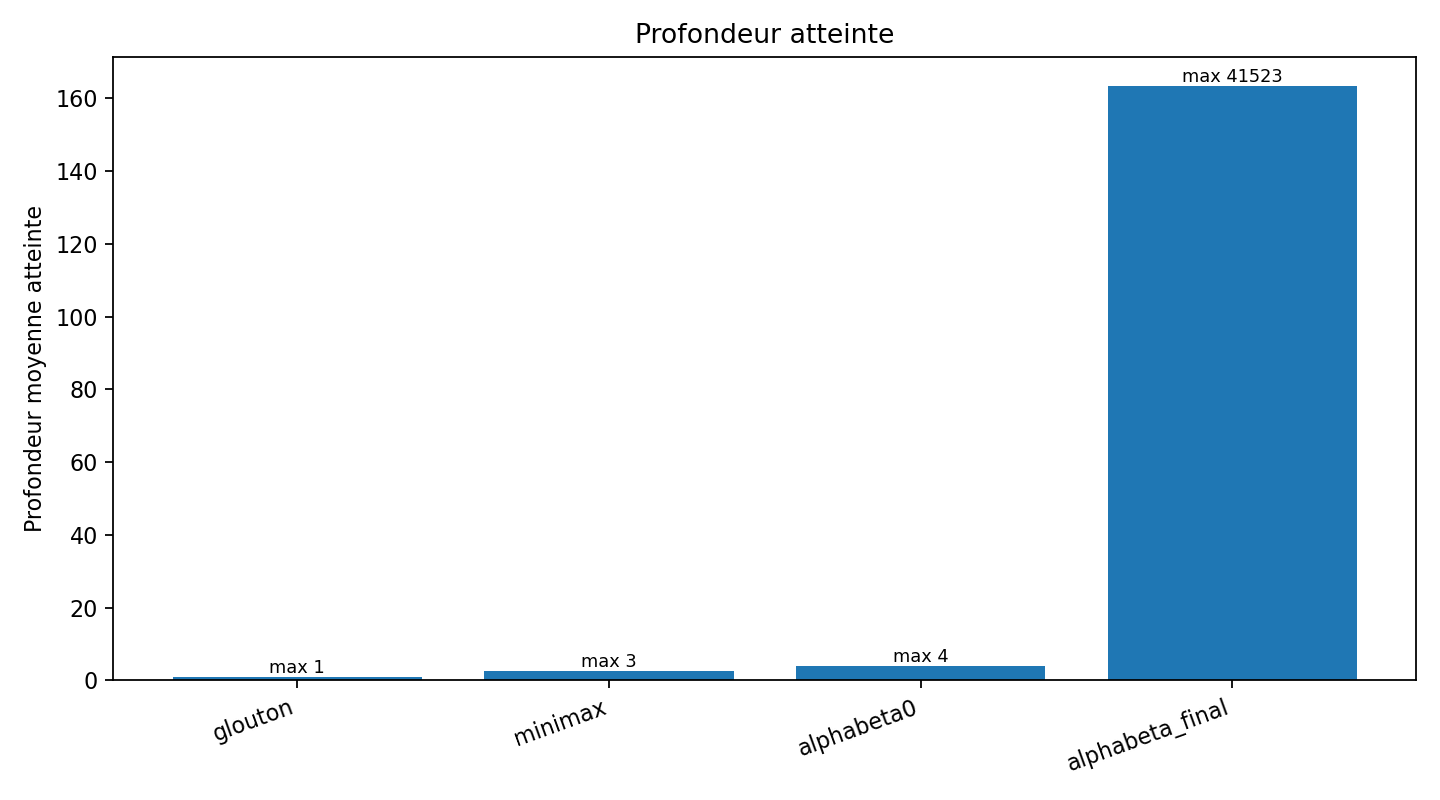
\includegraphics[width=\textwidth]{benchmark/results/graphs/depth_reached.png}
        \caption{Profondeur moyenne et maximale atteinte.}
        \label{fig:depth}
    \end{subfigure}\hfill
    \begin{subfigure}[b]{0.49\textwidth}
        \centering
        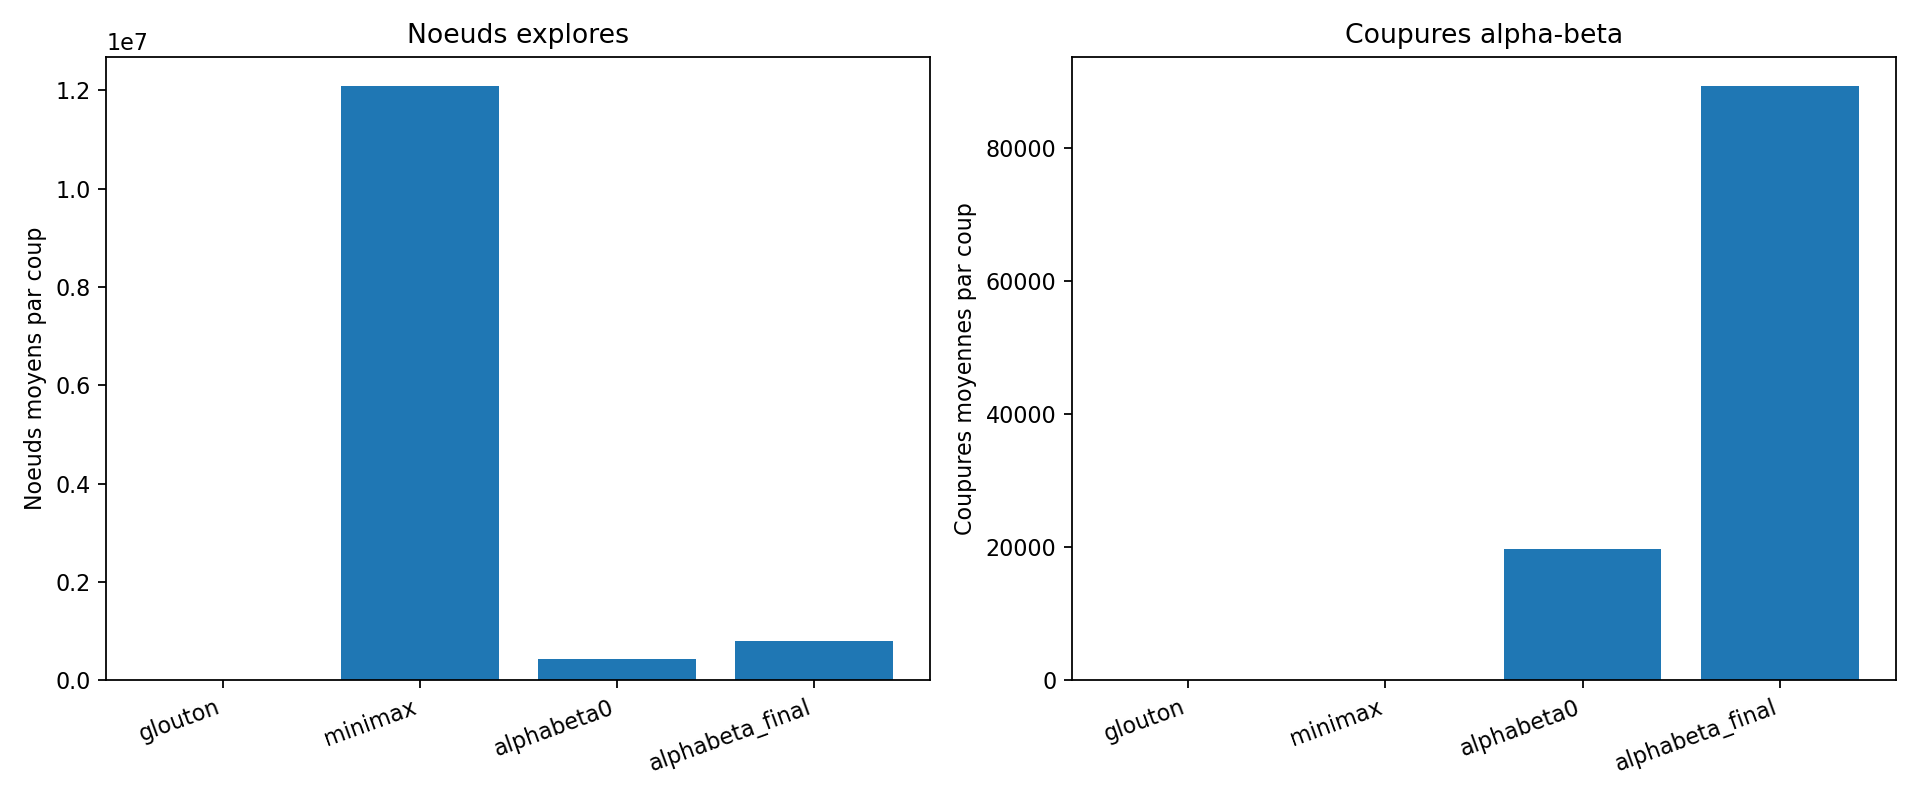
\includegraphics[width=\textwidth]{benchmark/results/graphs/nodes_and_cutoffs.png}
        \caption{Nombre moyen de noeuds explores et nombre moyen de coupures Alpha-Beta.}
        \label{fig:nodes-cutoffs}
    \end{subfigure}
    \caption{Profondeur atteinte (gauche) et travail exploratoire en noeuds/coupures (droite).}
\end{figure}

Les strategies a profondeur fixe, comme le Minimax et \texttt{alphabeta0}, ont une profondeur stable.
La version finale utilise l'approfondissement iteratif : la profondeur atteinte depend donc de la
position courante et du temps disponible. Le nombre de noeuds explores ne doit pas etre interprete seul :
une strategie peut explorer moins de noeuds mais obtenir de meilleurs resultats si le tri des coups
place les bons coups en premier et provoque davantage de coupures.

\subsection{Taux de victoire} 

\begin{figure}[H]
    \centering
    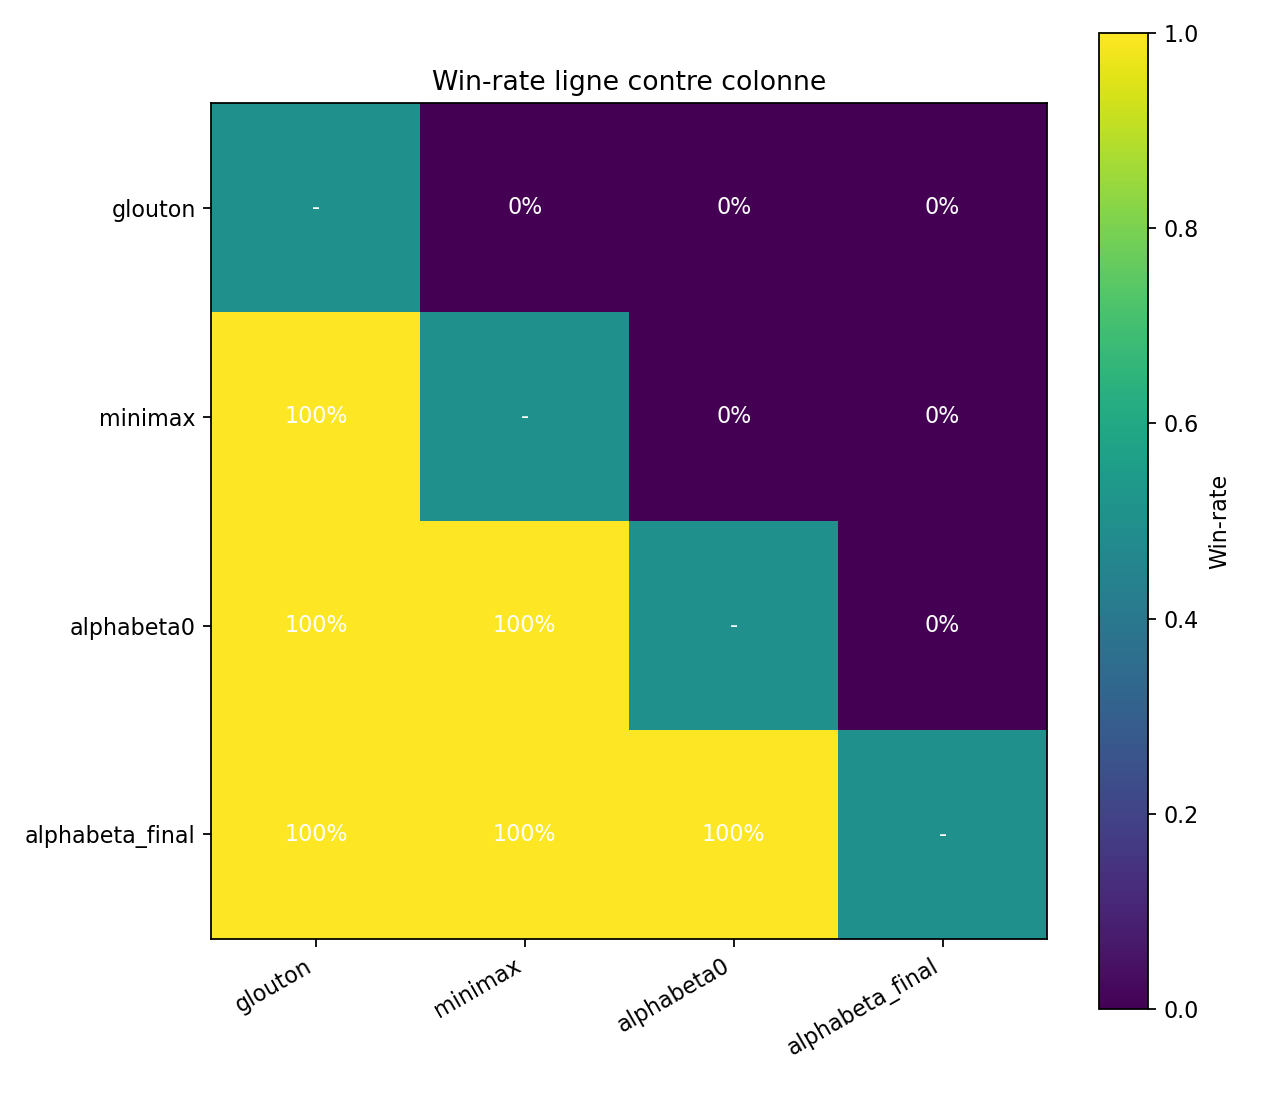
\includegraphics[width=0.75\textwidth]{benchmark/results/graphs/winrate_matrix.png}
    \caption{Win-rate ligne contre colonne.}
    \label{fig:winrate}
\end{figure}

Le taux de victoire est la mesure finale de qualite en situation de jeu. Nous testons les deux ordres
de depart, car une strategie peut se comporter differemment en tant
que joueur $1$ ou joueur $2$.

Globalement, le glouton est une baseline rapide mais myope : il peut choisir un gain immediat qui ouvre
une reponse adverse forte. Minimax corrige en partie ce defaut par l'anticipation, mais son cout
exponentiel devient vite limitant, meme a profondeur $3$. Alpha-Beta garde la meme logique de decision
que Minimax a profondeur egale, tout en reduisant le travail grace aux coupures ; son efficacite depend
fortement du tri des coups. La version finale ajoute enfin un parallelisme controle au niveau racine :
elle explore d'abord quelques bons coups pour obtenir une borne $\alpha$ utile, puis parallelise le reste,
ce qui evite une partie du surtravail d'un Alpha-Beta parallele trop naif.

\section{Conclusion}

Ce projet nous a permis de construire progressivement une intelligence artificielle pour Blob War.
La progression glouton, Minimax, Alpha-Beta puis Alpha-Beta parallele montre que la performance vient
surtout de la combinaison entre une bonne heuristique, un tri efficace des coups, des coupures nombreuses
et une gestion correcte du timeout par approfondissement iteratif. Des pistes restent ouvertes, notamment
les bitboards $64$ bits, les killer moves, Monte-Carlo/MCTS pour guider le tri et un work-stealing plus fin.

\end{document}
